\documentclass[titlepage,a4paper]{article}

\usepackage{a4wide}
\usepackage[colorlinks=true,linkcolor=black,urlcolor=blue,bookmarksopen=true]{hyperref}
\usepackage{bookmark}
\usepackage{fancyhdr}
\usepackage[spanish]{babel}
\usepackage[utf8]{inputenc}
\usepackage[T1]{fontenc}
\usepackage{graphicx}
\usepackage{float}

\graphicspath{ {imagenes/} }  % Las imagenes las reubique en la carpeta imagenes

\pagestyle{fancy} % Encabezado y pie de página
\fancyhf{}
\fancyhead[L]{TP1S - Max Mustermann}
\fancyhead[R]{Algoritmos y Programación III - FIUBA}
\renewcommand{\headrulewidth}{0.4pt}
\fancyfoot[C]{\thepage}
\renewcommand{\footrulewidth}{0.4pt}

\begin{document}
\begin{titlepage} % Carátula
	\hfill
\includegraphics[width=6cm]{logofiuba.jpg}
    \centering
    \vfill
    \Huge \textbf{Trabajo Práctico 1 — Smalltalk}
    \vskip2cm
    \Large [7507/9502] Algoritmos y Programación III\\
    Curso 2 \\ % Curso 1 para el de la tarde y 2 para el de la noche
    Primer cuatrimestre de 2020 
    \vfill
    \begin{tabular}{ | l | l | } % Datos del alumno
      \hline
      Alumno: & Paredes Ramirez, Luis Jose \\ \hline
      Número de padrón: & 104851 \\ \hline
      Email: & lparedesr@fi.uba.ar \\ \hline
  	\end{tabular}
    \vfill
    \vfill
\end{titlepage}

\tableofcontents % Índice general
\newpage

\section{Introducción}\label{sec:intro}
El presente informe reune la documentación de la solución del primer trabajo práctico de la materia Algoritmos y Programación III 
que consiste en desarrollar una aplicación de un sistema de una agencia de viajes en Pharo utilizando los conceptos del 
paradigma de la orientación a objetos vistos hasta ahora en el curso.

\section{Supuestos}\label{sec:supuestos}
% Deberá contener explicaciones de cada uno de los supuestos que el alumno haya tenido que adoptar a partir de 
% situaciones que no estén contempladas en la especificación.

Deberá contener explicaciones de cada uno de los supuestos 
que el alumno haya tenido que adoptar a partir de situaciones 
que no estén contempladas en la especificación.

  \begin{itemize}
    \item Del enunciado supongo que el pintor cobrara constantemente X cantidad por hora
    \item Otro supuesto
    \item Otro supuesto mas 
  \end{itemize}


\section{Diagramas de clase}\label{sec:diagramasdeclase}
% Uno o varios diagramas de clases mostrando las relaciones estáticas entre las clases. 
% Puede agregarse todo el texto necesario para aclarar y explicar su diseño. 
%Recuerden que la idea de todo el documento es que quede documentado y entendible cómo está implementada la solución.
Uno o varios diagramas de clases mostrando las relaciones estáticas entre las clases.  
Puede agregarse todo el texto necesario para aclarar y explicar su diseño. 
Recuerden que la idea de todo el documento es que quede documentado y entendible cómo está implementada la solución. 
Todos los diagramas tienen que estar embebidos como imágenes en el informe de manera tal que entren en el ancho de una hoja A4 
sin tener que rotarla.  No se aceptarán diagramas en archivos sueltos. 

%%%%%%%%%%%%%%%%%%%%%%%%%%%%%%%%%%%%%%%%%%%%%%%%%%%%%%%%%%% Cambiar  %%%%%%%%%%%%%%%%%%%%%%%%%%%%%%%%%%%%%%%%%%%%%%

\begin{figure}[H]
  \centering
  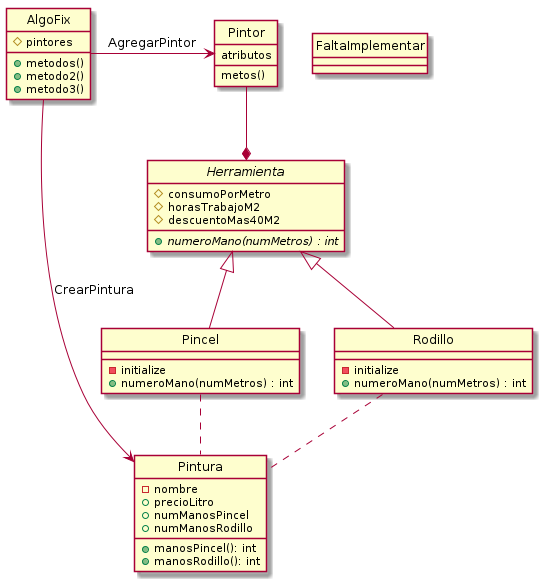
\includegraphics[width=0.8\textwidth]{test.png}
  \caption{\label{fig:class02}Prueba Diagrama de Clase.}
  \end{figure}

%%%%%%%%%%%%%%%%%%%%%%%%%%%%%%%%%%%%%%%%%%%%%%%%%%%%%%%%%%% Cambiar  %%%%%%%%%%%%%%%%%%%%%%%%%%%%%%%%%%%%%%%%%%%%%%

\begin{figure}[H]
\centering
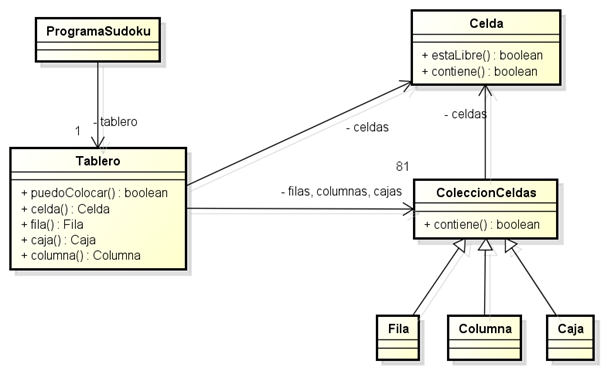
\includegraphics[width=0.8\textwidth]{diagrama_clase01.png}
\caption{\label{fig:class01}Diagrama del Sudoku.}
\end{figure}

\section{Detalles de implementación}\label{sec:implementacion}
% Explicaciones sobre la implementación interna de algunas clases que consideren que puedan llegar a resultar interesantes.
Explicaciones sobre la implementación interna de algunas clases que consideren que puedan llegar a resultar interesantes. 

\subsection{Subseccion 1}
Aca hay un codigo en Pharo

\begin{verbatim}
| rango |
rango := (2 to: 20) asOrderedCollection.
Transcript show: rango ; cr.
rango copy do: [ :unNumero | unNumero isPrime ifFalse: [ rango remove: unNumero ] ].
Transcript show: rango.
\end{verbatim}

\subsection{Subseccion 2}
Subseccion 2

\section{Excepciones}\label{sec:excepciones}
% Explicación de cada una de las excepciones creadas y con qué fin fueron creadas.

Explicación de cada una de las excepciones creadas y con qué fin fueron creadas (de manera concisa). 

\begin{description}
\item[Exception] 
\item[Excepcion] 
\item[Excepcion] 
\item[Excepcion]
\item[Excepcion]
\end{description}

\section{Diagramas de secuencia}\label{sec:diagramasdesecuencia}
% Mostrar las secuencias interesantes que hayan implementado. Pueden agregar texto para explicar si algo no queda claro.
Mostrar las secuencias interesantes que hayan implementado. Pueden agregar texto para explicar si algo no queda claro. 


\begin{figure}[H]
\centering
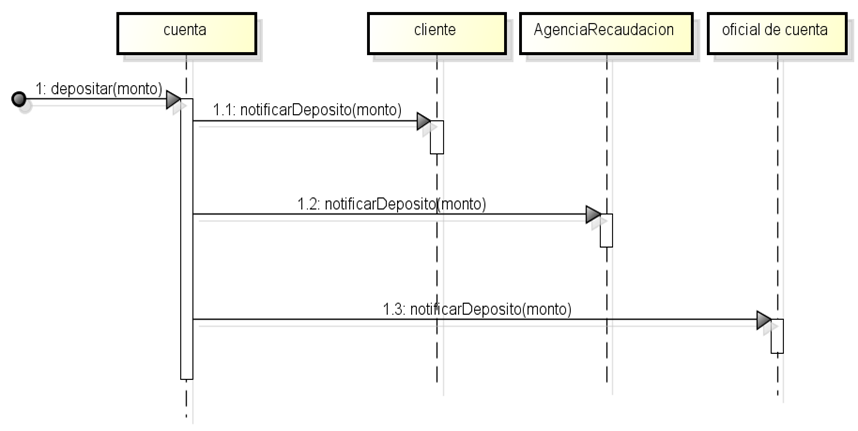
\includegraphics[width=0.8\textwidth]{diagrama_secuencia01.png}   %CAMBIAR ACA EL DIAGRAMA
\caption{\label{fig:seq01}Comportamiento esperado de depositar.}
\end{figure}

Implementar

\begin{figure}[H]
\centering
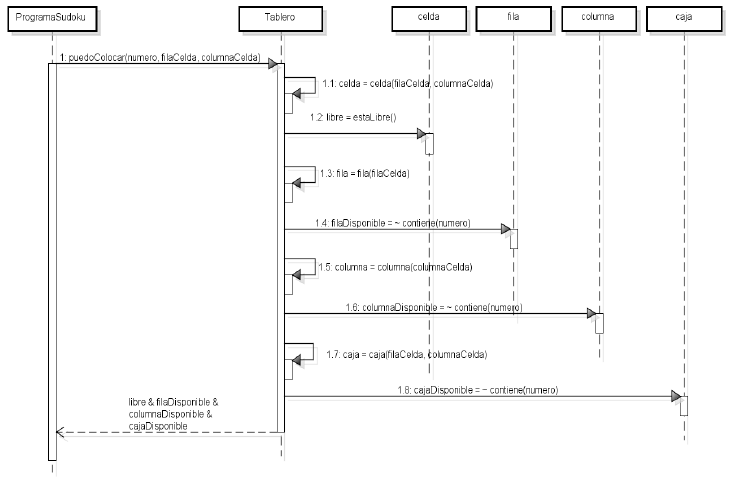
\includegraphics[width=\textwidth]{diagrama_secuencia02.png}
\caption{\label{fig:seq02}Diagrama de Secuencia de puedoColocar().}
\end{figure}

Implementar

\end{document}